\section{Continued Pre-Training for Cross-Game Control}
\label{sec:cpt}

Games differ in world, mechanics, and objectives, but most games share a unified device-level interface: screen observations and native keyboard and mouse inputs. As shown in Figure~\ref{fig:cpt_overview}, CPT adapts a pretrained multimodal model to this interface and learns transferable control from trajectories collected across environments. We first unify action representations across games and reduce biases caused by key frequencies and repeated control states. We then summarize findings from GameScaling~\cite{gamescaling} on how model capacity, gameplay data, and game composition affect control learning and cross-game generalization.

\begin{figure*}[!htbp]
    \centering
    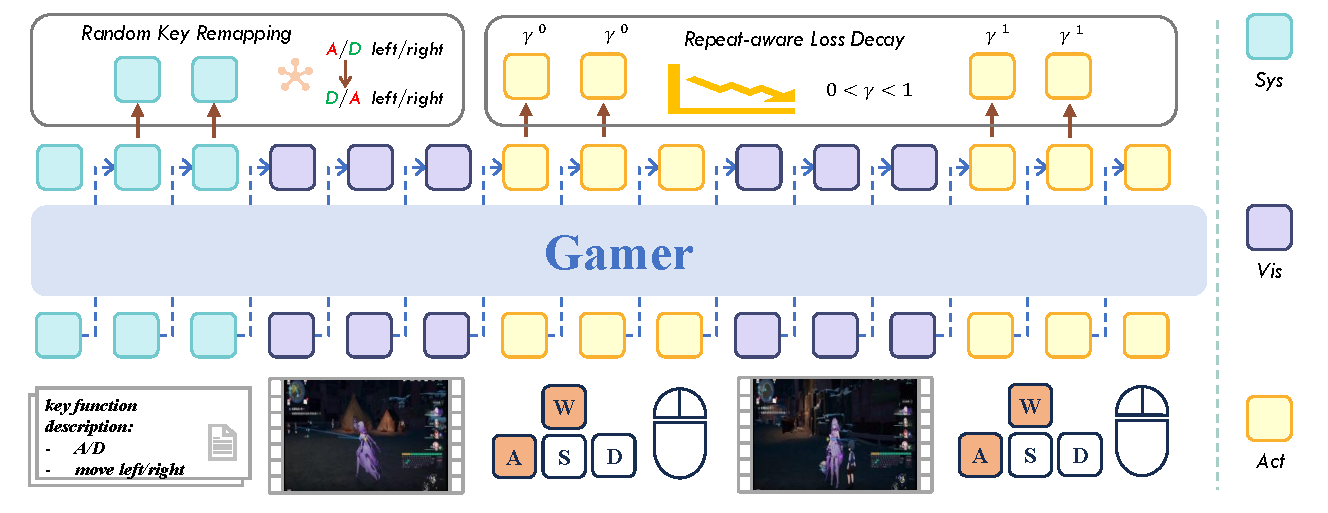
\includegraphics[width=0.88\linewidth]{figs/cpt.pdf}
    \caption{
    \textbf{CPT for unified keyboard-mouse control.}
    Synchronized gameplay observations and device events are mapped to a shared action representation. Random key remapping reduces reliance on key identity, while repeat-aware loss decay reweights temporally persistent actions. The resulting control prior is used by the subsequent task-conditioned training stages.
    }
    \label{fig:cpt_overview}
\end{figure*}

\subsection{Unified Observation-Action Representation}
\label{sec:unified_action}

Training across games requires a common action format that preserves the meaning of each game's controls. We represent each gameplay trajectory as interleaved screen observations and native keyboard-mouse actions. For each game, a control specification $\mathcal{B}$ maps physical inputs to their logical functions:
\[
\mathcal{B}=\{(k_i,d_i)\}_{i=1}^{|\mathcal{B}|},
\]
where $k_i$ is a keyboard key or mouse button and $d_i$ describes its in-game function. We include this specification in the policy input so that the model can interpret the shared input vocabulary using the target game's controls.

Following previous works~\cite{tan2025lumine,wang2025gametars}, we decouple visual decision making from low-level action execution. Observations are sampled every $200$\,ms ($5$\,Hz), and each observation interval is divided into six keyboard-mouse action blocks. Let $\mathcal{E}_t$ denote as the set of mouse movement events in interval $t$, where each event is represented by $\{ (\delta x_i,\delta y_i,\delta z_i)\}$, corresponding to horizontal movement, vertical movement, and scrolling, respectively. We define the action for interval $t$ as
\begin{equation}
a_t=\left(\Delta\mathbf{P}_t;\mathcal{K}_{t,1},\ldots,\mathcal{K}_{t,6}\right),
\qquad
\Delta\mathbf{P}_t=\sum_{\mathcal{E}_t}(\delta x_i,\delta y_i,\delta z_i),
\label{eq:action_representation}
\end{equation}
where $\Delta\mathbf{P}_t$ is the accumulated mouse movement in the interval $t$, and $\mathcal{K}_{t,j}$ ($j=1,\dots,6$) is the set of keyboard keys and mouse buttons pressed in action block $j$. We show more details of the action format in Figure~\ref{fig:action_format}. Each block lasts approximately $33$\,ms, yielding a $30$\,Hz action rate. Keys and buttons shared by consecutive blocks remain pressed, while those absent from the next block are released. This representation supports held movement, brief taps, dragging, and simultaneous input combinations without increasing the visual observation rate. Actions are serialized using the pretrained language model's output vocabulary, without an additional output head.

\begin{figure}[t]
    \centering
    \begin{tcolorbox}[
        enhanced,
        width=0.96\linewidth,
        colback=gray!6,
        colframe=black!65,
        boxrule=0.5pt,
        arc=1.2mm,
        left=3mm,right=3mm,top=4mm,bottom=3mm,
        title={Unified Keyboard-Mouse Action Serialization},
        fonttitle=\bfseries\normalsize,
        coltitle=white,colbacktitle=black!85
    ]
    \centering
    \normalsize\ttfamily
    \detokenize{<|action_start|>}
    $\Delta \mathbf{P}_t$
    \detokenize{;}
    $\mathcal{K}_1$
    \detokenize{;}
    $\mathcal{K}_2$
    \detokenize{;}
    $\mathcal{K}_3$
    \detokenize{;}
    $\mathcal{K}_4$
    \detokenize{;}
    $\mathcal{K}_5$
    \detokenize{;}
    $\mathcal{K}_6$
    \detokenize{<|action_end|>}
    \end{tcolorbox}
    \caption{\textbf{Serialized device-level action.} For each observation interval, the policy predicts accumulated mouse movement and six sequential sets of active keys and buttons.}
    \label{fig:action_format}
\end{figure}

Given $\mathcal{B}$ and a recent interaction history $\mathcal{H}_t$ containing the current observation and preceding observation-action pairs, the policy autoregressively generates an output sequence $y_t=[r_t, a_t]$:
\begin{equation}
\pi_\theta(y_t\mid\mathcal{B},\mathcal{H}_t)
=\prod_{j=1}^{|y_t|}
\pi_\theta(y_{t,j}\mid\mathcal{B},\mathcal{H}_t,y_{t,<j}),
\label{eq:autoregressive_policy}
\end{equation}
where $r_t$ is an optional reasoning sequence preceding the executable action $a_t$, and  $y_{t,j}$ is the $j$-th output token. For a small fraction of CPT turns, $r_t$ contains retrospective reasoning annotated from the observation and recorded action. These annotations preserve the backbone's optional reason-then-act format without changing the action targets. The same executable action representation is retained during SFT, online RL, and deployment.

\subsection{Trajectory Debiasing and Temporal Reweighting}
\label{sec:trajectory_debiasing}

Gameplay data exhibit two biases that can limit transferable control learning. Uneven key frequencies encourage the model to associate actions with specific inputs rather than their functions, while long runs of repeated actions can dominate the token-level supervision. We address these biases with random key remapping and repeat-aware loss decay, respectively.

\paragraph{Random key remapping.}
For each trajectory, we sample a random bijection $\sigma:\mathcal{K}_{\mathrm{bind}}\rightarrow\mathcal{K}_{\mathrm{bind}}$ over rebindable keys. Inputs with fixed semantics remain unchanged. The same mapping is applied to the control specification and the actions:
\begin{equation}
\begin{aligned}
\mathcal{B}^\sigma
  =\{(\sigma(k_i),d_i)\}_{i=1}^{|\mathcal{B}|},\quad
\mathcal{K}_{t,j}^\sigma
=\{\sigma(k)\mid k\in\mathcal{K}_{t,j}\},\quad
a_t^\sigma
    =\left(\Delta\mathbf{P}_t; \mathcal{K}_{t,1}^\sigma,\ldots,\mathcal{K}_{t,6}^\sigma\right).
\end{aligned}
\end{equation}
Historical actions are remapped consistently to obtain $\mathcal{H}_t^\sigma$, whereas visual observations and mouse displacements remain unchanged. The policy is trained to predict $a_t^\sigma \sim \pi_\theta(a_t^\sigma\mid\mathcal{B}^\sigma,\mathcal{H}_t^\sigma)$. The mapping remains fixed within a trajectory, preserving its control semantics while reducing shortcuts based on frequent key identities.

\paragraph{Repeat-aware loss decay.}
More than $85\%$ of the action steps in our interaction data repeat the preceding action, which is common in gameplay since players often hold the same inputs across multiple time steps to perform sustained behaviors such as moving or waiting. These repetitions record how long such behaviors last, so we retain the full trajectories while reducing the contribution of prolonged repetitions. Following the decaying-loss formulation in Game-TARS~\cite{wang2025gametars}, we down-weight consecutive repeated actions. Specifically, the action-token component of the CPT objective we used is
\begin{equation}
\begin{aligned}
\mathcal{L}_{\mathrm{action}}
    &=-\sum_{t=1}^{T}\omega_t
      \sum_{j=1}^{|a_t|}
      \log\pi_\theta(a_{t,j}\mid\mathcal{B},\mathcal{H}_t,r_t,a_{t,<j}),\quad
\omega_t=\gamma^{n_t-1},
\end{aligned}
\label{eq:cpt_objective_1}
\end{equation}
where $n_t$ counts consecutive repetitions of the current action and resets to $1$ whenever the action changes. We use $\gamma=0.9$ and omit the remapping superscript for clarity. When present, retrospective reasoning tokens are additionally supervised as part of the same autoregressive response. Eq.~\eqref{eq:cpt_objective_1} specifies the reweighting applied to action tokens, not the full mixed-token objective.

A newly issued action receives full weight, while successive repetitions contribute progressively less. This preserves action duration while emphasizing behavior transitions, such as stopping, turning, and interacting. Random key remapping discourages reliance on key identity, while repeat-aware decay shifts supervision toward changes in behavior.

The CPT objective combines the reweighted action-token loss with a standard autoregressive loss for the optional reasoning tokens:
\begin{equation}
\begin{aligned}
\mathcal{L}_{\mathrm{CPT}}
&=\mathcal{L}_{\mathrm{action}}+\mathcal{L}_{\mathrm{reason}},\\
\mathcal{L}_{\mathrm{reason}}
&=-\sum_{t=1}^{T}
\sum_{j=1}^{|r_t|}
\log\pi_\theta(r_{t,j}\mid\mathcal{B},\mathcal{H}_t,r_{t,<j}).
\end{aligned}
\label{eq:cpt_objective}
\end{equation}
Here, $r_t=\varnothing$ for turns without reasoning, so the corresponding reasoning loss is zero. The repeat-aware weight $\omega_t$ is applied only to action tokens. For clarity, we omit the remapping superscript; when key remapping is applied, the control specification, interaction history, and action targets are remapped consistently.

\subsection{Scaling Laws and Cross-Game Generalization}
\label{sec:cpt_scaling}

Although a shared control interface makes cross-game CPT possible, the benefits of additional gameplay data depend on how well the training data cover the target environment. GameScaling \cite{gamescaling} examines this dependence by varying model size, gameplay budget, and game composition. We summarize its findings here to contextualize Gamer’s CPT stage.

To characterize these effects, a composition-aware scaling relation based on D-CPT Law~\cite{que2024dcpt} is adopted. Let $N$ be model size, $D$ the gameplay budget in hours, and $q\in[0,1]$ the proportion of gameplay relevant to a specified validation distribution. The validation loss is modeled as
\begin{equation}
\mathcal{L}_{\mathrm{val}}(N,D,q)
=E+\frac{C_N}{N^a}
+\frac{C_D q^\eta}{D^b}
+\frac{C_q}{(q+\epsilon)^c},
\label{eq:cpt_scaling_law}
\end{equation}
where $E$, $C_N$, $C_D$, $C_q$, $a$, $b$, $c$, and $\eta$ are fitted variables. The small constant $\epsilon>0$ keeps the expression finite when the target game's share is zero. In view of the widespread use of Minecraft in prior work~\cite{wang2025gametars,fan2022minedojo}, Gamescaling \cite{gamescaling} varies its proportion in the gameplay mixture to study the effect of data composition. We use $q=w_{\mathrm{MC}}$ for Minecraft validation and $q=1-w_{\mathrm{MC}}$ for validation over the remaining training-game distribution, where $w_{\mathrm{MC}}$ is the Minecraft fraction of the gameplay mixture.

The data term describes how validation loss changes with the gameplay budget, and the final term captures differences between data mixtures. The scaling relation fits the training-game distributions and supports held-out prediction within the measured range. However, distant unseen games do not exhibit sustained gains from additional CPT data. Sec.~\ref{sec:exp_cpt_scaling} provides the controlled study and its empirical limits. CPT thus provides transferable control, while more distant worlds and longer tasks motivate additional task-conditioned supervision and online interaction.